\chapter{Experimental constraints}
\label{ch:ExConst}
There is a plethora of experimental searches for dark matter. Some of the applicable to the leptophilic models considered here will be presented in this section. 
\section{Four lepton Z decay}
The decay of the Z boson to four leptons has been studied with ATLAS detector at the LHC. 
\begin{figure}[H]
\centering
\begin{tikzpicture}
\begin{feynman}
\vertex (a) {\(\bar{q}\)};
\vertex [above right=1.41cm of a](c);
\vertex [above=2cm of a](b) {\(q\)};
\vertex [right=of c](d);
\vertex [below right=of d](e);
\vertex [above right=3cm of d](f1){\(l^-\)};
\vertex [below right=3cm of d](f4){\(l^+\)};
\vertex [above right=of e](g);
\vertex [above right= 1cm of g](f2){\(l^-\)};
\vertex [below right= 1cm of g](f3){\(l^+\)};

\diagram* {
(b) -- [fermion](c) -- [fermion] (a),
(c) -- [boson,edge label=\(Z/\gamma\)](d),
(f4) --[fermion](d) --[fermion](f1),
(f3) --[fermion](g) --[fermion](f2),
(e) --[boson,edge label=\(A'/Z/\gamma\)](g)
};
\end{feynman}
\end{tikzpicture}
\caption{Four lepton Z decay as a SM process (Z/$\gamma$) and BSM process (A')}
\label{fg:ZtoFourL}
\end{figure}
At the Z resonance, this process is dominated by the s-channel diagram shown in figure \ref{fg:ZtoFourL}.
This results in 
\begin{equation}
BR(\text{Z}\rightarrow 4l) = (3.20\pm 0.25 (\text{stat})\pm 0.13 (\text{syst}))\cdot 10^{-6}
\end{equation}
and is again consistent with the standard model \cite{Aad:2014wra}. This can be used to constrain the parameter space for new couplings. For example the Z' in the diagram shown above contibutes to the decay beyond the SM. But the techiques of the analysis only allow a narrow window of $5\text{ GeV} \lesssim m_{Z'}\lesssim 50 \text{ GeV}$ to be constrained \cite{Altmannshofer:2014pba}. This is mainly due to the cut on the dilepton invariant mass of $m_{l^+l^-}>5\text{ GeV}$.
\section{Neutrino trident production} 
Neutrino trident production is a process in which neutrinos are scattering of the coulomb field of the target material. The leading contributions come from a Photon coupling between the nucleus and the charged lepton and Z and W bosons coupling to the neutrino (see figure \ref{fg:trident}) and are thus suppressed. In addition, the destructive interference between diagrams with W and Z bosons suppress the SM process even further. 
\begin{figure}[H]
\centering
\begin{tikzpicture}
\begin{feynman}
\vertex (a1);
\vertex [above=0.2cm of a1](a2);
\vertex [above=0.2cm of a2](a3);
\vertex [right=3cm of a1](b1);
\vertex [right=3cm of a2](b2);
\vertex [right=3cm of a3](b3);
\vertex [right=3cm of b1](c1);
\vertex [right=3cm of b2](c2);
\vertex [right=3cm of b3](c3);
\vertex [above right=1.5cm of b3](d);

\vertex [above=0.5cm of d](e);


\vertex [above left=1.5cm of e](h1);
\vertex [left=3cm of h1](g1){\(\nu_\mu\)};
\vertex [right=3cm of h1](g2){\(\nu_\mu\)};
\vertex [above=0.5cm of c3](f1){\(\mu^-\)};
\vertex [below=0.5cm of g2](f2){\(\mu^+\)};;
\diagram* {
(a1) -- [fermion](b1) -- [fermion](c1),
(a2) -- [fermion](b2) -- [fermion](c2),
(a3) -- [fermion](b3) -- [fermion](c3),
(b3) -- [boson,edge label=\(\gamma\)](d),
(f2) --[fermion](e) -- [fermion](d) -- [fermion](f1),
(g1) -- [fermion](h1) -- [fermion](g2),
(e) -- [boson,edge label=\(Z/A'\)](h1)
};
\draw [decoration={brace}, decorate] (a1.south west) -- (a3.north west)
node [pos=0.5, left] {\(N\)};
\draw [decoration={brace}, decorate] (c3.south west) -- (c1.north west)
node [pos=0.5, right] {\(N\)};
\end{feynman}
\end{tikzpicture}
\caption{Neutrino-trident graph as a SM process (Z) and BSM process (A')}
\label{fg:trident}
\end{figure}
The CHARM-II collaboration and the CCFR collaboration both measured the crossection width a $\sim 20$ GeV beam on glass and $\sim 160$ GeV beam on an iron target respectively \cite{Altmannshofer:2014pba}.
The reported cross-sections relative to the SM-predictions are:
\begin{align*}
\frac{\sigma_\text{CHARM-II}}{\sigma_\text{SM}}&=1.58\pm 0.57\\
\frac{\sigma_\text{CCFR}}{\sigma_\text{SM}}&=0.82\pm0.28
\end{align*}
Bounds obtained for the cross section here can be used to obtain constraints on vectorial couplings to the muon and muon-neutrino for gauged $L_\mu-L_\tau$ or $L_e-L_\mu$ models. 
\section{Beam Dump Experiments}
One way to produce a vector mediator at a fixed target experiment is by the production of neutral pions or eta mesons  $p+p\rightarrow X+\pi^0/\eta$ that subsequently decays to $\pi^0/\eta\rightarrow A' + \gamma$ by the diagram shown in figure \ref{fg:BeamDumpPion}
\begin{figure}[H]
\centering
\begin{tikzpicture}
\begin{feynman}
\vertex (a1){\(\pi^0/\eta\)};
\vertex [right=2cm of a1](b);
\vertex [above right=2cm of b](c1);
\vertex [below right=2cm of b](c2);
\vertex [right=2cm of c1](f1){\(\gamma\)};
\vertex [right=2cm of c2](f2){\(A'\)};

\diagram* {
(a1) -- [scalar](b),
(b)--[fermion](c1)--[fermion](c2)--[fermion](b),
(c1)--[boson](f1),
(c2)--[boson](f2)
};
\end{feynman}
\end{tikzpicture}
\caption{Neutral meson decay to A' and $\gamma$ by kinetic mixing}
\label{fg:BeamDumpPion}
\end{figure}
The resulting branching ratio can then be related to that of the standard model radiative decay to two photons \cite{deNiverville:2011it}:
\begin{equation}
Br(\pi^0/\eta \rightarrow \gamma A')= 2\epsilon^2\left(1-\frac{m_{A'}^2}{m_{\pi/\eta}^2}\right)^3 Br(\pi^0/\eta \rightarrow \gamma\gamma)  .
\end{equation}
This can then be immediately be used to search for monophoton final states or simply missing energy.
Another way to use the resulting mediators is to utilise its decay products $\chi$ if the decay is allowed and rapid enough. The resulting $\chi$ beam can then be used to constrain the model by its scattering shown in the following diagram:
\begin{figure}[H]
\centering
\begin{tikzpicture}
\begin{feynman}
\vertex (a1);
\vertex [above=0.1cm of a1](a2);
\vertex [right=2cm of a1](b1);
\vertex [right=2cm of a2](b2);
\vertex [right=2cm of b1](c1);
\vertex [right=2cm of b2](c2){\(e/N\)};
\vertex [above=2cm of a2](a3){\(\chi\)};
\vertex [right=2cm of a3](b3);
\vertex [right=2cm of b3](c3){\(\chi\)};
 \node[above=1cm of b2, crossed dot] (d) {};


\diagram* {
(a1) -- [fermion](b1)--[fermion](c1),
(a2) -- [fermion](b2)--[fermion](c2),
(a3) -- [fermion](b3)--[fermion](c3),
(b2) --[boson,edge label=\(\gamma\)](d)--[boson,edge label=\(A'\)](b3)
};
\end{feynman}
\end{tikzpicture}
\caption{$\chi$ scattering on either electrons or nuclei.}
\label{fg:ChiScattering}
\end{figure}
These processes can be investigated with the data sets taken by the LSND and MiniBooNE experiments. Their data sets for the analysis of neutrino scattering can be used to constrain the parameter space, because the $\chi$-scattering leads to a similar signature. 
The case where the dark photon decays to an electron pair has been investigated by the NA48/2 experiment at CERN. Here an irreducible background comes from the standard model Dalitz decay. The resulting bounds on $\epsilon$ are shown in figure \ref{fg:NA48Bounds}.
\begin{figure}[H]
  \centering
    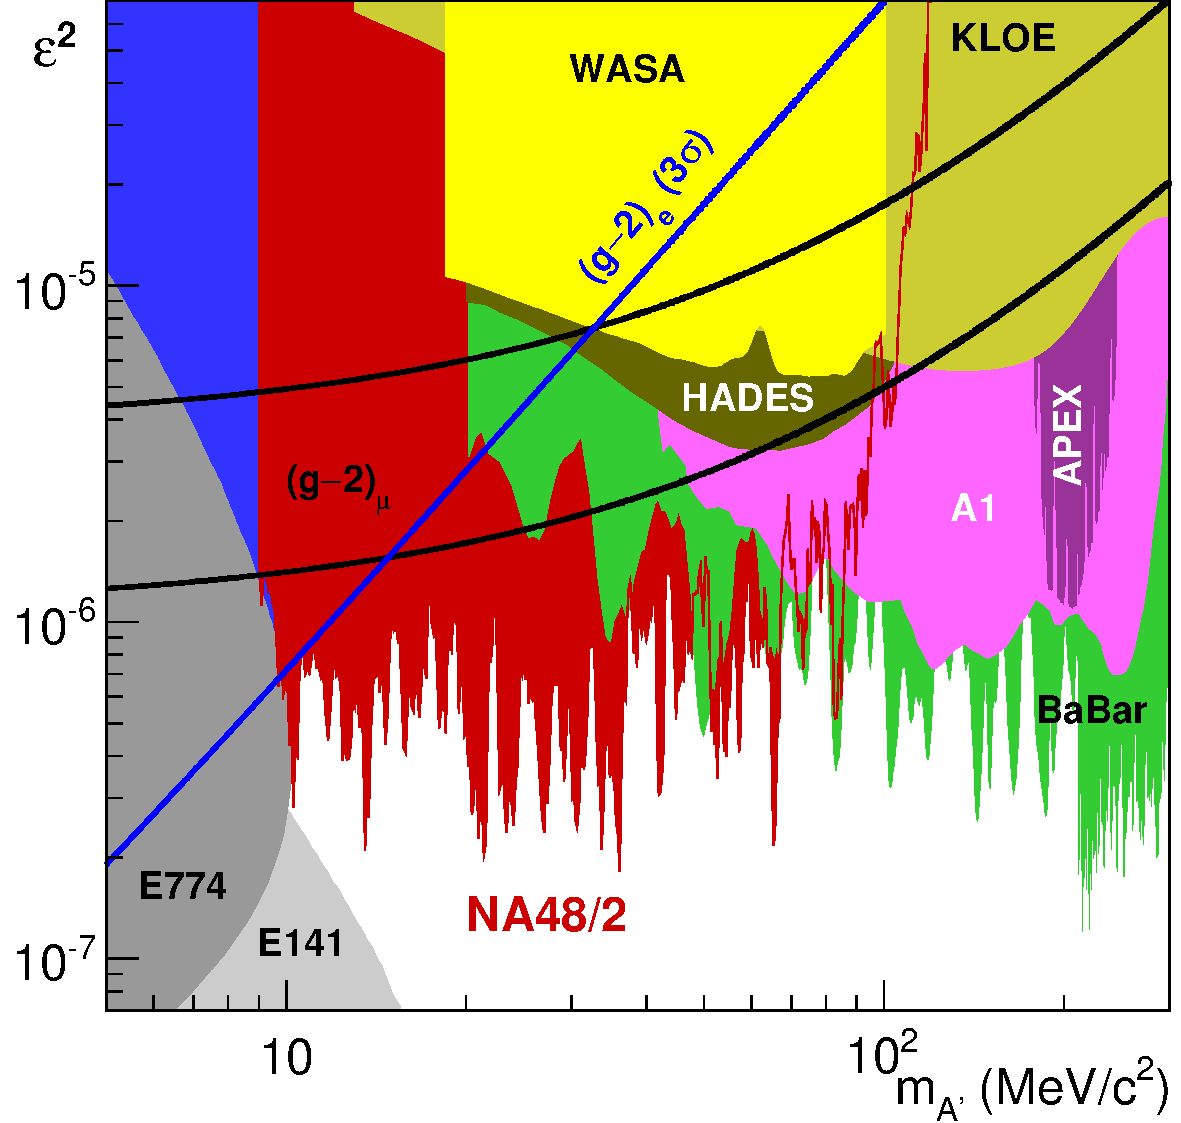
\includegraphics[width=0.4\textwidth]{imgs/dp_exclusion}
    \caption{Upper limits at 90\% CL on $\epsilon^2$ from \cite{Lurkin:2017aqo}}
    \label{fg:NA48Bounds}
\end{figure}
Although this result is only valid for pure kinetically mixed dark photons without the direct lepton coupling this can be used to construct the corresponding bound on $e'_l$ with the assumption that $\epsilon$ is absent at tree level by using equation \ref{eq:KinMix}.

\paragraph{NA64}
Another experiment that is used to constrain the dark photon models is NA64 at CERN SPS that dumps an electron beam on a target detector. Among the standard model particle shower, a dark photon might be created as bremsstrahlung shown in figure \ref{fg:DP-Porduction}. The possible detection is then by the large missing energy, that the dark photon carries away when it decays invisibly. The corresponding bound is shown in figure \ref{fg:BABAR}. The kinetic mixing parameter $\epsilon$ can in this case be identified with the direct electron coupling by $e_e'=e\epsilon$.

\begin{figure}[H]
\centering
\begin{tikzpicture}
\begin{feynman}
\vertex (a1);
\vertex [above=0.1cm of a1](a2);
\vertex [right=2cm of a1](b1);
\vertex [right=2cm of a2](b2);
\vertex [right=2cm of b1](c1);
\vertex [right=2cm of b2](c2){\(N\)};
\vertex [above=2cm of a2](a3){\(e\)};
\vertex [right=2cm of a3](b3);
\vertex [right=1.6cm of a3](c);
\vertex [right=2cm of b3](c3){\(e\)};
\vertex	[above=0.8cm of c3](f1){\(A'\)};


\diagram* {
(a1) -- [fermion](b1)--[fermion](c1),
(a2) -- [fermion](b2)--[fermion](c2),
(a3) -- [fermion](b3)--[fermion](c3),
(b2) --[boson,edge label=\(\gamma\)](b3),
(c) -- [boson](f1)
};
\end{feynman}
\end{tikzpicture}
\caption{Dark photon production as bremsstrahlung}
\label{fg:DP-Porduction}
\end{figure}
\section{\texorpdfstring{$e^+ e^-$}{e+e-} collider}
Another direct search for the dark photon has been carried out by the BABAR Collaboration. This experiment used collision data from the PEP-II B-factory and looked for events with one high energy photon with large missing momentum. This would receive a contribution from $e^+e^-\rightarrow \gamma A'$ where the dark photon decays invisibly to the dark sector. The collaboration established 90\% C.L. bounds on the mixing parameter of the kinetically mixed photon. Again this can straight forwardly be generalised to the model for the direct coupling to the leptons where $e_e'=e\epsilon$.
\begin{figure}[H]
  \centering
    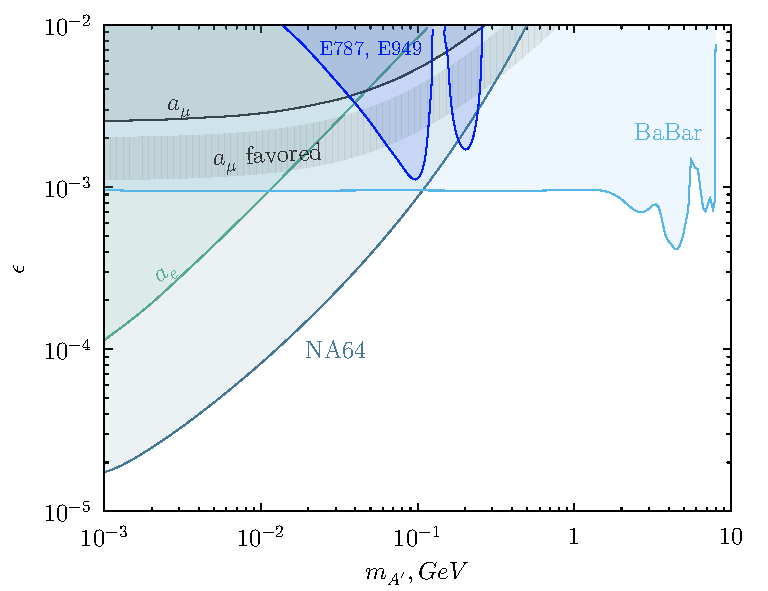
\includegraphics[width=0.6\textwidth]{imgs/exclusionInvisible-1909}
    \caption{BABAR and NA64 Upper limits at 90\% CL on $\epsilon$ from \cite{Banerjee:2018vgk}}
    \label{fg:BABAR}
\end{figure}
\section{Atomic Physics}
\paragraph{1S-2S transition in positronium}
Exotic atoms made of only leptons are a great place to test predictions from QED, because in contrast to hydrogen, the constituents are fundamental particles themselves. This avoids uncertainties like the internal structure of the proton in hydrogen, that affects the energy levels. 
If a new scalar field with mass $m_\phi$ that couples to particles i and j is introduced, it gives rise to a Yukawa potential of the form \cite{Frugiuele:2019drl}
\begin{equation}
V^{ij}(r)= -\frac{e'_i e'_j}{4\pi}\frac{e^{-m_\phi r}}{r}.
\end{equation}
This gives rise to energy shifts in atom like objects that contain particles i and j. The coupling to the electron on its own can be probed in bound states with multiple electrons that are at the same time well understood such as positronium and helium. For example the current standard model prediction and experimental measurement of the 1S-2S transition in positronium are:
\begin{align}
(E(2^3S_1)-E(1^3S_1))_{\text{Ps}}^\text{th}&=1233607222.13(58)\text{MHz}\\
(E(2^3S_1)-E(1^3S_1))_{\text{Ps}}^\text{exp}&=1233607216.4(3.2) \text{MHz}
\end{align}
The requirements that these deviate less than $2\sigma$ results in the bounds shown in figure \ref{fg:AtomicElectronBound}. Also included are bounds from the electron anomalous magnetic moment. This will be ignored in the further discussion because the contribution from two additional fields may cancel and render this bound deceiving. 

\begin{figure}[H]
\centering
\begin{subfigure}{.5\textwidth}
  \centering
  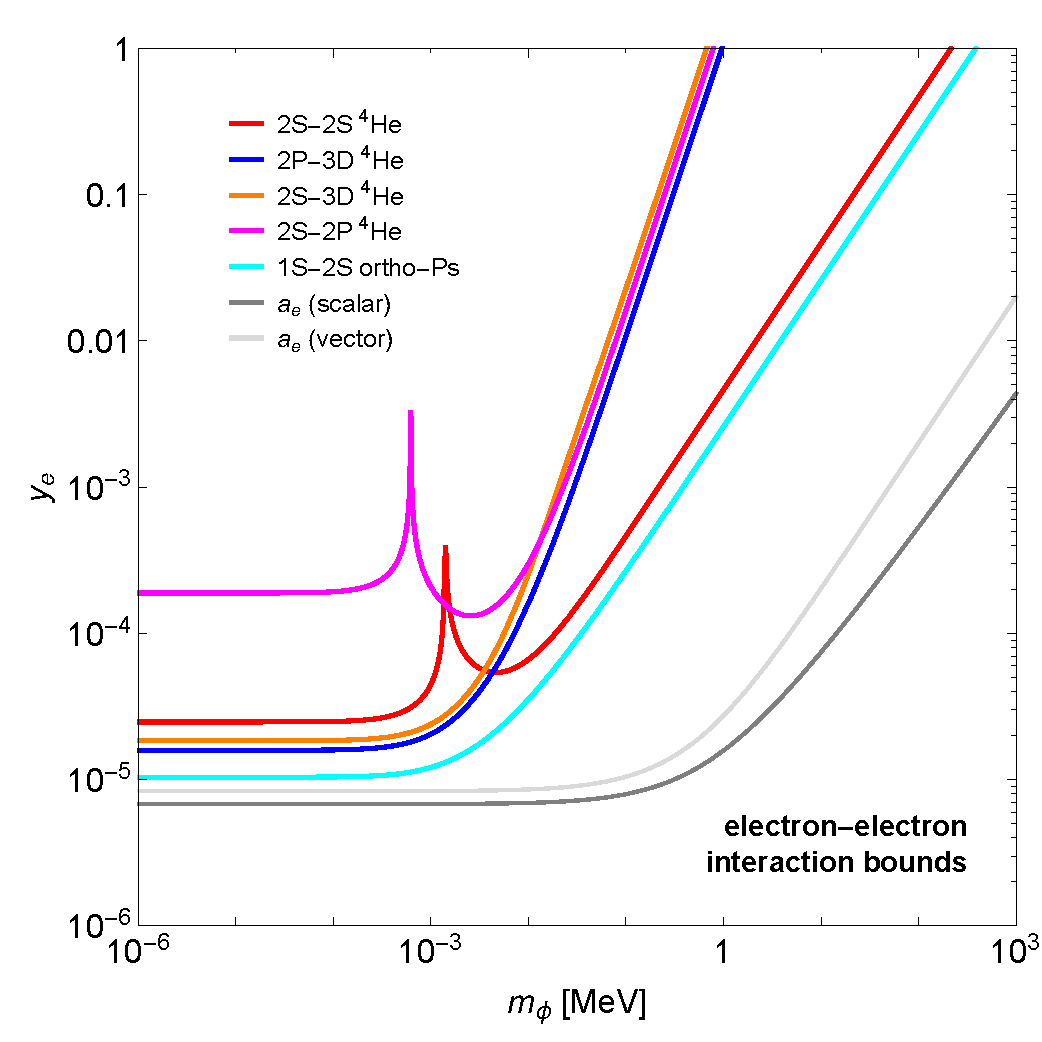
\includegraphics[width=\linewidth]{imgs/yebound-final}
  \caption{Upper limits on $y_e = e'_e$}
\end{subfigure}%
\begin{subfigure}{.5\textwidth}
  \centering
  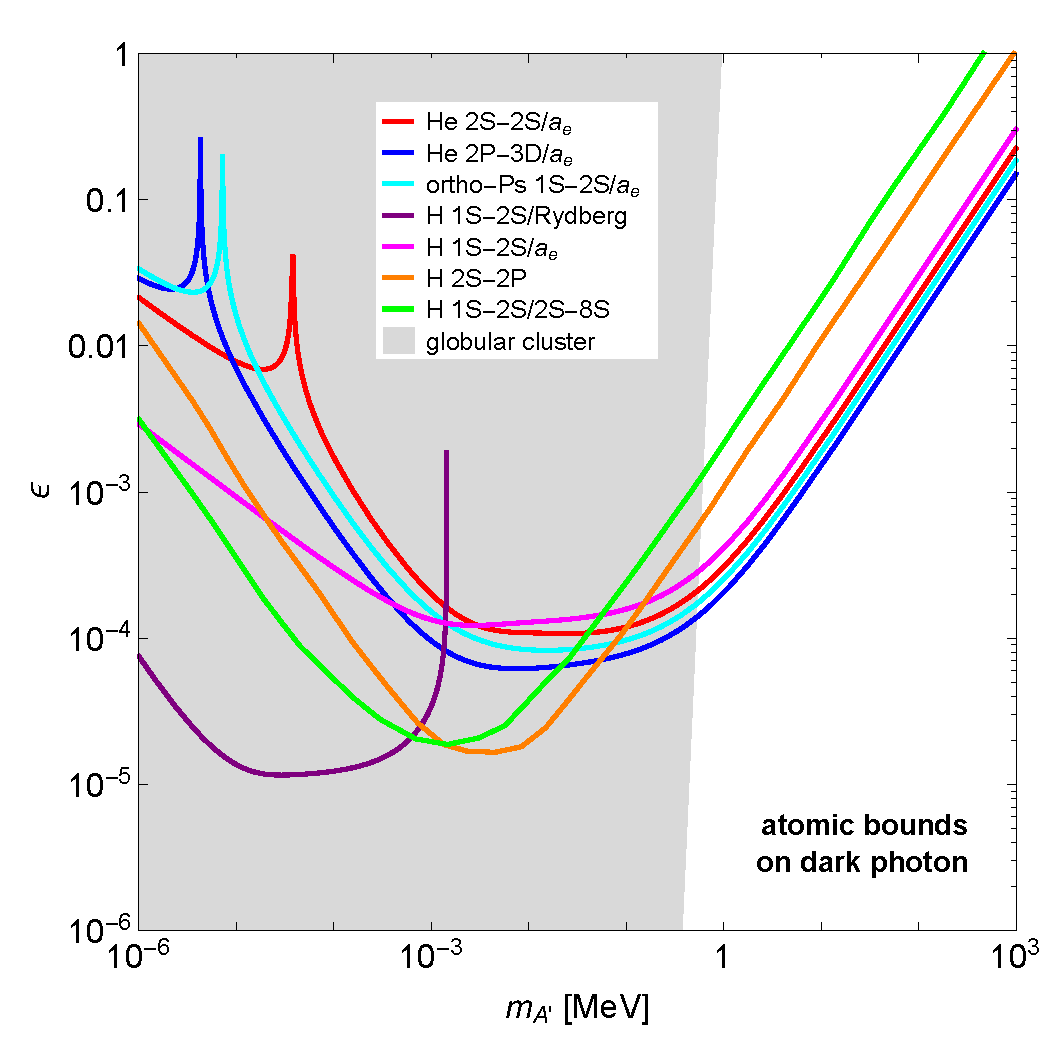
\includegraphics[width=\linewidth]{imgs/DP-final}
  \caption{Upper limits on $\epsilon$}
\end{subfigure}
\caption{Taken from \cite{Delaunay:2017dku} }
\label{fg:AtomicElectronBound}
\end{figure}

\paragraph{Muonium}
The other coupling relevant to this work is to the muon. Sadly the direct analogue to the previous paragraph consisting of only muons, the true muonium has neither been measured nor even been seen. The alternative is the spectrum of muonium, that is despite of its name a bound state of an electron and an anti-muon. The theoretical and experimental values for the 1S-2S transitions for this case are:
\begin{align}
(E(2S_1)-E(1S_1))_{\text{Mu}}^\text{th}&=2455528941.0(9.8)\text{MHz}\\
(E(2S_1)-E(1S_1))_{\text{Mu}}^\text{exp}&=2455528935.8(1.4) \text{MHz}.
\end{align}
Special care has to be taken to evaluate the theoretical value, because the 1S-2S transition is used to calculate $m_\mu/m_e$ which in turn sets the muon mass, so it's not independent on the BSM influence. 
Also the lamb shift in muonium has been calculated and measured to :
\begin{align*}
(E(2S_{1/2})-E(2P_{1/2})_\text{Mu}^\text{th}&=1047.284(2)\text{MHz}\\
(E(2S_{1/2})-E(2P_{1/2})_\text{Mu}^\text{exp}&=1042(22)\text{MHz}
\end{align*}
Both can seperately be used to construct bound on the product of couplings $e'_\mu e'_e=g_e\times g_\mu$ \cite{Frugiuele:2019drl} These are shown in figure \ref{fg:MuoniumBounds}
\begin{figure}[H]
  \centering
    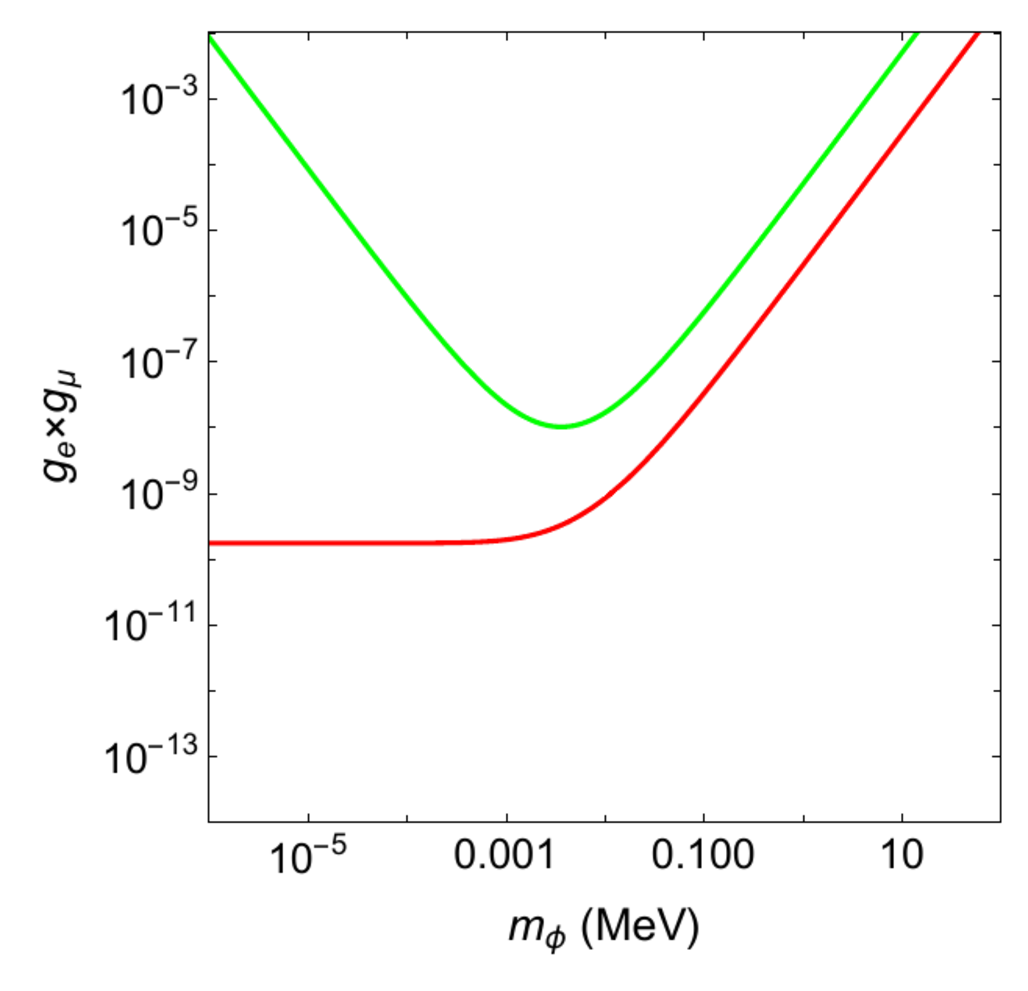
\includegraphics[width=0.5\textwidth]{imgs/muonium1}
    \caption{Upper limits at 95\% CL on $g_e\times g_\mu$ from Mu 1S-2S transition (red) and the Lamb shift (green). Taken from \cite{Frugiuele:2019drl}}
    \label{fg:MuoniumBounds}
\end{figure}
\section{Future Experiments}
\paragraph{Belle II}
Belle II is an experiment at the SuperKEKB $e^+e^-$collider in Japan that started data acquisition in early 2018. Even though its main use is as a B-factory to study B-meson properties, it will also serve as a test ground for electrophilic new physics. Its data set will allow stronger constraints to the electron dark photon coupling in mono photon events with a photon energy of $E_\gamma = \frac{s-M_{A'}^2}{2\sqrt{s}}$ when the dark photon is produces on shell and escapes the detector/ decays to the dark sector, or additionally with two opposite leptons with a center of mass energy of the dark photon mass when it decays to the standard model leptons. 
In either case the bounds on the kinetic mixing parameter can be straight forwardly be converted to the direct lepton coupling models. To reach higher sensitivity for these events, the upgrade from Belle to Belle II included a single photon trigger ans is going to run at a higher luminosity.\cite{Inguglia:2016acz}.  
\paragraph{NA64-\texorpdfstring{$\mu$}{mu}}
Since the NA64-experiment is run only with electrons and only searches for dark photon decays to an $e^+e^-$ pair, its insensitive to any coupling to muons. To remedy this and explore the $(g-2)_\mu$ anomaly further, the $NA64_\mu$-run is proposed and if its approved is scheduled to run after 2021. Here a $\mu^+$-beam on target is used to search for an excess of missing momentum events where the muon is slightly scattered that points to the bremsstrahlung production of a mediator with subsequent invisible decay. Among the gauged $L_\mu-L_\tau$ this might be most useful for scalar mediators coupling to muons.
\paragraph{$M^3$: Muon Missing Momentum Experiment}
$M^3$ is a proposed experiment at Fermilab where a $\SI{15}{\giga \eV}$ muon beam impacts an active target. Then signatures for $\mu N \rightarrow \mu N \slashed{E}$ are searched. In this case the missing energy $\slashed{E}$ comes from the invisible decay of the mediator coupled to the muon that is produced by bremsstrahlung. In phase 1 this is then proposed to deliver bounds on the scalar coupling of $<3\dot10^{-4}$ and on the vector coupling of  $<2\dot10^{-4}$ for masses below $\SI{100}{\mega \eV}$ \cite{Kahn:2018cqs}.